% a sample file for Journal of Quantum Information and Computation (QIC) in 
% LaTex2e by inputing macro file "qic.sty" with command \usepackage{qic}, 
% all the macros have been defined in the style file, so it is no need to 
% put many macros at the beginning of the text file  

\documentclass[twoside]{article}
\usepackage{qic,epsfig}
\usepackage{braket}
\usepackage{bm}
\usepackage{amssymb}
\usepackage{amsmath}
\usepackage{cancel}
\usepackage{qcircuit}
\usepackage{mathtools}
\usepackage{verbatim}
\usepackage{breqn}
\usepackage{tikz}
\usepackage{url}
\usetikzlibrary{arrows.meta}

\textwidth=5.6truein
\textheight=8.0truein

\renewcommand{\thefootnote}{\fnsymbol{footnote}}  %use symbolic footnote

%%%%%%% starting the text file 

\begin{document}
\setlength{\textheight}{8.0truein}    %FOR 2ND PAGE ONWARDS

\runninghead{Mapping Fermions to Qubits  $\ldots$}
            {Oliver O'Brien $\ldots$}

\normalsize\textlineskip
\thispagestyle{empty}
\setcounter{page}{1}

%\copyrightheading{Vol.}{No.}{Year}{Page Nos.}

  

\alphfootnote

\fpage{1}

\centerline{\bf
%%%%%%%%%%%%%%%%%%%%%
%Put in titiles here
%%%%%%%%%%%%%%%%%%%%%
MAPPING FERMIONS TO QUBITS}
\vspace*{0.37truein}
\centerline{\footnotesize 
%%%%%%%%%%%%%%%%%%%%%%%%%%%%%%%%%%%%
%put authors' name and address here
%%%%%%%%%%%%%%%%%%%%%%%%%%%%%%%%%%%%
OLIVER O'BRIEN}
\vspace*{0.015truein}
\centerline{\footnotesize\it DAMTP, Centre for Mathematical Sciences, University of Cambridge, Cambridge CB30WA, UK}
\baselineskip=10pt
\centerline{\footnotesize\it Christ's College, Cambridge, UK}
\vspace*{0.225truein}
\publisher{(received date)}{(revised date)}

\vspace*{0.21truein} 

%% \abstracts{first paragraph}{second paragraph}{third paragraph}
%% If there is only one paragraph, just keep the second and third empty 
%% like the following one 
\abstracts{
%%%%%%%%%%%%%%%%%%%%
% put abstract here
%%%%%%%%%%%%%%%%%%%%
Your abstract goes here. 
}{}{}

\vspace*{10pt}

\keywords{The contents of the keywords}
\vspace*{3pt}
\communicate{to be filled by the Editorial}

\vspace*{1pt}\textlineskip    %) USE THIS MEASUREMENT WHEN THERE IS
   %) A SECTION HEADING
%\vspace*{-0.5pt}
%\noindent
%%%%%%%%%%%%%%%%%%%%%%%%%%%%%%%%
%put the text of the paper here
%%%%%%%%%%%%%%%%%%%%%%%%%%%%%%%%
\section{Introduction}
"Nature isn't classical, dammit, and if you want to make a simulation of nature, you'd better make it quantum mechanical, and by golly it's a wonderful problem, because it doesn't look so easy." - \textsl{Dr Richard Feynman} \cite{feynmann}  \\\\
Ever since Dr Richard Feynman spoke these famous words at the end of his keynote speech in 1982 one of the main tasks facing quantum computers has been simulating quantum systems. Intuitively a quantum computer should be able to handle this problem better than a classic computer as they operate within the same bizarre world of entanglement and superposition. However, there are many challenges to overcome before quantum advantage can be achieved in this field. We will consider one such challenge in this essay: the optimum mapping scheme from fermions to qubits.\\\\
One of the most common classes of quantum systems we wish to simulate are those composed of fermions. In order to simulate these particles we must find a representation for them a quantum computer can process; in terms of qubits and qubit operators. This poses a fundamental issue as fermions exhibit the non-local property of anti-commutation (\textbf{need to explain why this is non-local}), whereas qubits are independent local units (\textbf{they may be independent and local but could they not just be half-spin particles instead}). Therefore a non-trivial mapping scheme which introduces this non-local behaviour is necessary.\\\\
The first such mapping, the \textbf{Jordan-Wigner Transformation}, was invented nearly a century ago \cite{originalJordanWigner}, and we will introduce it in Section~\ref{jordan-wigner_section}. More recently, a number of new mappings have been developed including the \textbf{Bravyi-Kitaev map} and the \textbf{Derby-Klassen map}, which will be discussed in Section~\ref{bravyi-kitaev_section} and Section~\ref{derby-klassen_section} respectively. Furthermore, recent research \cite{fermionicEncoding} has shown that the \textbf{fermionic enumeration} scheme used in a given mapping (we consider solely the Jordan-Wigner case) offers potential for increased locality with no additional resources. This is elaborated on in Section~\ref{fermionic-enumeration_section}.\\\\
It is important to consider how these mappings impact upon the fermionic simulation techniques used. Therefore, in Section~\ref{applications_section} (below) we will discuss how VQE and phase estimation can both be used to estimate the ground state energy of a system. Finally,  in Section~\ref{comparision_section} we will compare the relative performance of these mappings in real-world applications (using simulated quantum computers).
\section{Applications to fermionic systems}\label{applications_section}
\subsection{Estimating ground state energies}\label{vqe_section}
Computing the ground state energy of a Hamiltonian is generally the first step in computing the energetic properties of molecules and materials \cite{vqe}. Chemists have developed classical computational models for estimating the ground state, however, they all rely on approximations. Quantum computing opens up the potential for an exact (\textit{full configuration interaction}) approach, which is unfeasible on a classical computer where it scales exponentially (\textbf{verify this is true}) in the number of fermionic modes.
\subsubsection{Variational Quantum Eigensolver}
A VQE provides an upper bound on the ground state energy of a Hamiltonian by utilising the variational principle:
\begin{equation}
        \frac{\bra{\psi} \hat H \ket{\psi}}{\braket{\psi | \psi}} \geq E_0 \>\>\>\> \forall \> \ket{\psi}\in \mathcal{H}
\end{equation}
The algorithm consists of two stages. First a variational ansatz $\ket{\psi}$ is initialised based on a set of parameters $\bm \theta$. Then, the Hamiltonian is measured a number of times, and the parameters of the ansatz are varied (using a classical optimiser) until a minimum is found. This is an example of a variational quantum algorithm, which performs a classical optimisation over a quantum oracle (\textbf{is this a correct description}). By exporting lots of the work to a classical computer, VQEs are one of the quantum algorithms that are achievable in the NISQ (Noisy Intermediate-scale Quantum) era.\\\\ 
The preparation of ansatz can be done without any regard for fermions or what underlying wavefunction it represents. Generally a given circuit structure is picked with some of the gates depending upon the parameters (i.e. an $R_z(\theta)$ gate). However, there are some schemes for preparing ansatz that correlate to known wavefunctions, so the wavefunction corresponding to the minimum energy estimate can be found (\textbf{check this is true, find example and see if mapping is important} - Unitary Coupled Cluser - gaussian).\\\\
It is in the measurement of the Hamiltonian that the mapping becomes important. The Hamiltonian in question will be a combination of fermionic raising and lowering operators, so needs to be mapped to a combination of Pauli operators that can be measured on a quantum computer. \textbf{consider measurement strategies that minimise repetitions}. After this mapping has been performed we are left with a qubit Hamiltonian that is a sum of Pauli strings (strings of Pauli operators). Therefore, we can measure the effectiveness of different mappings by the resource costs of implementing this qubit Hamiltonian. We will focus on three metrics (\textbf{this bit might be too similar to \cite{vqe} page 31\cite{vqe}}):
\begin{romanlist}
\item \textbf{Number of qubits:} The less qubits required by the mapping the smaller the quantum computer required to run the simulation.
\item \textbf{Average Pauli weight:} The average number of Pauli operators in each Pauli string in the Hamiltonian. The smaller the Pauli weight the less gates needed to measure the Hamiltonian, which reduces both the resource cost and the error due to gate infidelity. \textbf{Low-weight operators protect against barren plateau} \url{doi:10.1038/s41467-021-21728-w.}. \textbf{Could potentially elaborate here as it is a bit more complex than just less gates per string it also increases parallelisation (so reduces depth) and reduces ansatz depth}. \textbf{Mention locality}
\item \textbf{Number of Pauli-strings:} Each Pauli-string is measured separately, so the fewer Pauli-strings to measure, the fewer times the ansatz needs to be initialized and measured.
\end{romanlist}
\subsubsection{Quantum Phase estimation} \label{qpe_section}
QPE can be used to estimate the energy levels of a Hamiltonian to $n$ bits. This is achieved by applying successive steps of time evolution as a controlled gate with the target being the input state and the control being successive Hadamard ancilla qubits (illustrated in Fig.~\ref{QPECircuit}). Then by performing an inverse Quantum Fourier Transform on these ancilla qubits we get a superposition of binary expressions for the energy levels.\\
\begin{figure}[htbp]
               \centerline{ \Qcircuit @C=1em @R=.7em {
                               \lstick{\ket{0}} & \gate{H} & \qw            & \qw              & \qw              & \qw              & \qw &  \cdots &                & \ctrl{8}           & \qw & \multigate{7}{QFT^{-1}} & \qw \\ \\ \lstick{\cdots} & \cdots  & \cdots & \cdots & \cdots &\cdots &  & \cdots & &  & \cdots& & \cdots  \\   \\
                               \lstick{\ket{0}} & \gate{H} & \qw            & \qw              & \qw              & \ctrl{4}         & \qw &  \cdots &                & \qw                & \qw & \ghost{QFT^{-1}}& \qw  \\
                               \lstick{\ket{0}} & \gate{H} & \qw            & \qw              & \ctrl{3}         & \qw              & \qw &  \cdots &                & \qw                & \qw & \ghost{QFT^{-1}}& \qw   \\
                               \lstick{\ket{0}} & \gate{H} & \qw            & \ctrl{2}         & \qw              & \qw              & \qw &  \cdots &                & \qw                & \qw & \ghost{QFT^{-1}}& \qw   \\
                               \lstick{\ket{0}} & \gate{H} & \ctrl{1}       & \qw              & \qw              & \qw              & \qw &  \cdots &                & \qw                & \qw & \ghost{QFT^{-1}}& \qw   \\
                               \lstick{\ket{u}} & \qw      & \gate{U^{2^0}} & \gate{U^{2^{1}}} & \gate{U^{2^{2}}} & \gate{U^{2^{3}}} & \qw &  \cdots &                & \gate{U^{2^{n-1}}} & \qw & \qw & \qw
        }}
        \vspace*{13pt}
        \fcaption{\label{QPECircuit} Circuit diagram of QPE. In order to calcualte energy levels $U = e^{-2\pi i \hat H}$ is used.}
\end{figure} \\
An important feature of the algorithm is that the guiding state $\ket{u}$ must have overlap with the ground state. This can be seen by working through in detail (the following treatment is adapted from \cite{chemistryReview}):\\
\begin{itemlist}
\item We can express $\ket{u}$ in the basis of energy eigenstates: $\ket{u} = \sum_i c_i \ket{E_i}$. Therefore, the total state after the application of the Hadamard gates is: 
        \begin{equation}
                \frac{1}{\sqrt{2^n}} \sum_i \sum_x \ket{x} c_i \ket{E_i}
        \end{equation}
\item After the application of the controlled gates shown in Fig.~\ref{QPECircuit}, this transforms to:
        \begin{equation}
        \frac{1}{\sqrt{2^n}} \sum_i c_i (\ket{0} + e^{-2\pi i  E_i 2^0}\ket{1})(\ket{0} + e^{-2\pi i E_i 2^1} \ket{1}) \cdots (\ket{0} + e^{-2\pi i  E_i 2^{n-1}}\ket{1}) \ket{E_i} \end{equation}
        as $x = x_0 2^0 + x_1 2^1 + \cdots + x_{n-1} 2^{n-1}$ for $x_i \in \{0,1\}$, this reduces to:
        \begin{equation}
                \frac{1}{\sqrt{2^n}} \sum_i \sum_x e^{-2\pi i E_i x}c_i \ket{x}  \ket{E_i}
        \end{equation}
\item By applying an inverse Fourier transform the phase can be extracted:
        \begin{equation}
                \frac{1}{\sqrt{2^n}} \sum_i \sum_x e^{-2\pi i E_i x}c_i \ket{x}  \ket{E_i} \xrightarrow{QFT^{-1}} \sum_i c_i \ket{\text{bin}(E_i)} \ket{E_i}
        \end{equation}
\item As $E_i$ is likely not exact to $n$ bits there will be a potential error introduced by the Quantum Fourier Transform, so to be accurate to $n$ bits a few more ancilla qubits will be needed \cite{nielsenChuang}.
\item By measuring the ancilla bits in the Z basis we will observe $E_i$ to $n$ bits with probability $|c_i|^2$.  So to find the ground state energy level, the ground state eigenstate needs to be in the original expansion of the guiding state $\ket{u}$. The larger the amplitude of the ground state eigenstate ($c_0$) the fewer repetitions of QPE are required before $E_0$ is measured. Therefore, QPE works better if a guiding state close to the exact ground state is used. \textbf{Why is this section here it does not seem relevant to the topic}
\end{itemlist}
The portion of this algorithm for which fermionic mapping is relevant is the construction of the controlled gates $U^{2^k} = e^{-2 \pi i \hat H 2^k}$. Not only do the same metrics for the efficiency of the corresponding qubit Hamiltonian listed in Section~\ref{vqe_section} apply, now we need to consider the impact of exponentiation. As the Hamiltonian is the sum of non-commuting Pauli-strings taking the exponential is non-trivial and requires the Trotter-Suzuki approximation \cite{suzuki}. To first order this gives:
\begin{equation}
        e^{\frac{-it}{\hbar} \sum^m_k \hat H_k} = \left( \prod^m_k e^{\frac{-i t \hat H_k}{\hbar S}}\right)^S + O(t^2/S)
\end{equation}
In order to achieve a desired accuracy of $\epsilon$ a sufficient number of Trotter steps $S= O(t^2/ \epsilon)$ need to be used \cite{chemistryReview}. The ordering of the terms in this Trotter-Suzuki expansion greatly influences the error and therefore how many Trotter steps are required. This is important to consider as the impact the ordering has varies depending on the mapping chosen as we will discuss in Section~\ref{comparision_section}.\\\\
Finally, it is useful to consider how each Trotter step is represented as a circuit. First, we consider that $e^{i(Z_1 \otimes Z_2 \otimes ... \otimes Z_n)\theta}$ applies a phase shift of $e^{i\theta}$ if the parity of the $n$ qubits is even and $e^{-i\theta}$ if the parity is odd \textbf{don't actually state or justify how this expression is represented as a circuit}. Secondly, it is possible to transform $e^{i(Z_1 \otimes Z_2 \otimes ... \otimes Z_n)\theta}$ into the exponentiation of any Pauli-string by applying $R_X$ or Hadamard gates to change the basis to the X or Y basis, respectively. Therefore, in general the exponential of a $n$-fold tensor product of Pauli matrices will require $2(n-1)$ CNOT gates centred around one phase-shift gate and enough $R_X$ and Hadamard gates to transform into and out of the necessary basis before and after \cite{seeley}. As an example the circuit required for computing the term $e^{i(YXZY)\theta}$ is shown in Fig.~\ref{trotterStepCircuit}. As such it is clear that each Trotter step requires gates linear in \textbf{is it the pauli weight or the total pauli weight ?? this whole section needs reconsidering now ive done the course} \begin{figure}[htbp]
\centerline{ \Qcircuit @C=1em @R=.7em {
        &\gate{R_X} & \ctrl{1} & \qw & \qw & \qw & \qw & \qw & \ctrl{1} & \gate{R_X^{\dagger}}&\qw \\
        &\gate{H} & \targ & \ctrl{1} & \qw & \qw & \qw & \ctrl{1} & \targ & \gate{H}& \qw\\
        & \qw & \qw & \targ & \ctrl{1} & \qw & \ctrl{1} & \targ & \qw & \qw &  \qw\\
        &\gate{R_X} & \qw & \qw & \targ & \gate{R_Z(2 \theta)} & \targ & \qw & \qw & \gate{R_X^{\dagger}} &\qw \\
}}
        \vspace*{13pt}
        \fcaption{\label{trotterStepCircuit} The circuit required to exponentiate the Pauli-string $YXZY$ by first converting the qubits into the correct basis using $R_X$ and $H$ gates, then computing the parity of the four qubits before applying a single-qubit phase rotation. After this we uncompute the parity and revert to the computational (Z) basis. This is adapted from \cite{seeley}.}
\end{figure}
\subsection{Simulating dynamics - see Nielsen Cheung}
\section{First and second quantization}
\textbf{This section needs rewriting it is too confusing - in particular need to address what role qubits are actually playing here (dirac notation needs some words around it)}
From Quantum Field Theory (\textbf{citation needed}), we know that fermions must be antisymmetric under exchange. This property is commonly represented by qubits in two ways known as the first and second quantization. The first quantization is when the antisymmetry is retained in the wavefunction such as with:
\begin{equation}\label{antisym}
        \ket{\Phi} = \frac{1}{\sqrt{2}}(\ket{\phi}_1 \ket{\psi}_2 - \ket{\psi}_1 \ket{\phi}_2)
\end{equation}
We can generalise Eq.~\ref{antisym} to larger numbers of fermions through a Slater determinant (Eq.~\ref{slater}) \cite{chemistryReview}. This satisfies the antisymmetry condition as swapping any two rows of a determinant produces a sign change:
\begin{equation}\label{slater}
        \phi(\bm x_0, ..., \bm x_{N-1}) = \frac{1}{\sqrt{N!}} 
        \begin{vmatrix} 
                \phi_0(\bm x_0) & \cdots & \phi_{M-1}(\bm x_0)\\
                \vdots & \ddots & \vdots \\
                \phi_0(\bm x_{N-1}) & \cdots & \phi_{M-1}(\bm x_{N-1})
        \end{vmatrix}
\end{equation}
Here $M$ is the number of spin orbitals possible, and $N$ is the number of electrons. Typically we have more spin orbitals than electrons, so the Slater determinant will only contain the $N$ occupied spin orbitals. Acting with fermionic creation and annihilation operators on the first quantization is trivial (if long-winded) as the operators either commute with or act upon each mode. \\\\
The second quantisation compresses the information of the Slater determinant by only tracking whether each orbital or fermionic mode is occupied. Therefore the above is written as:
\begin{equation}
        \phi(\bm x_0, ..., \bm x_{N-1}) = \ket{f_0,\cdots, f_i, \cdots, f_{M-1}}
\end{equation}
where $f_i$ (the occupation number) $ =1$ when $\phi_p$ is occupied, and 0 otherwise. This is termed the Fock basis. Acting on the Fock basis with the fermionic creation and annihilation is more complex and is given by \cite{chemistryReview}:
\begin{equation}
        \label{secondQuant}
        \begin{align}
        a_p \ket{f_0,\cdots, f_i, \cdots, f_{M-1}} = \delta_{f_p, 1} (-1)^{\sum_{i=0}^{p-1} f_i} \ket{f_0,\cdots, f_p \oplus 1, \cdots, f_{M-1}}\\
        a_p^{\dagger} \ket{f_0,\cdots, f_i, \cdots, f_{M-1}} = \delta_{f_p, 0} (-1)^{\sum_{i=0}^{p-1} f_i} \ket{f_0,\cdots, f_p \oplus 1, \cdots, f_{M-1}}
\end{align}
\end{equation}
Therefore, second quantization can be thought of as encoding the antisymmetry of the fermions in the operators rather than the quantum states. All the mappings we will consider are examples of encoding second quantization (\textbf{should I consider first quantisation techniques}).\\\\
\textbf{explain advantages of second quantisation vqe chemistry review tranter 2015}
\section{Jordan-Wigner Transformation}\label{jordan-wigner_section}
The Jordan-Wigner transformation straightforwardly stores the occupation number of the $i$-th orbital in the $i$-th qubit. Therefore, all the non-local behaviour (the parity information) has to be encoded in the operators \cite{fermionicEncoding}:
\begin{equation}
        \begin{align}
        a_i \rightarrow \left( \bigotimes_{k=1}^{i-1} Z_k \right) \sigma_i^-\\
        a^{\dagger}_i \rightarrow \left( \bigotimes_{k=1}^{i-1} Z_k \right) \sigma_i^+
\end{align}
\end{equation}
where
\begin{equation}
        \begin{align}
                \sigma^-_i = \frac{1}{2} (X_i + i Y_i) = \ket{0}_i \bra{1}_i\\
                \sigma^+_i = \frac{1}{2} (X_i - i Y_i) = \ket{1}_i \bra{0}_i 
        \end{align}
\end{equation}
It is clear to see that these operators act in exactly the same way on a qubit spin basis that the fermionic creation and annihilation operators act upon the Fock basis. \textbf{might be worth explaining why the naive approach doesn't work and hence the motivation for the $Z_k$s}
\section{Bravyi-Kiteav Map}\label{bravyi-kitaev_section}
The Jordan-Wigner transformation uses O(1) qubits to represent each fermionic mode, however it requires O(N) gates to simulate one fermionic operation. This is because it stores the occupation number locally and the parity non-locally. An alternative scheme called the parity basis stores the parity locally and the occupation number non-locally, however this still requires O(N) gates to simulate one fermionic operation \cite{seeley}. The Bravyi-Kiteav is a halfway house which partially stores both the occupation number and parity non-locally.\\\\
We will describe three different formulations of the mapping: partial ordering, transformation matrices and Fenwick trees. The partial ordering scheme was that first used by Bravyi and Kiteav \cite{bravyikitaev} and provides the clearest illustration of operator locality. Transformation matrices are intuitively easier to understand, but the complexity is less clear. The following explanation of the mapping is adapted from \cite{bravyikitaev}. (\textbf{maybe also talk about Fenwick trees \cite{operatorLocality}}). First, we must define a partial order $\preceq$ over a set of binary strings. For $\alpha = \alpha_{l-1}\ldots \alpha_0$ and $\beta = \beta_{l-1}\ldots \beta_0$, if $\alpha_i = \beta_i$ for $i\geq i_0$ and $\beta_i = 1$ for $i < i_0$, then $\alpha \preceq \beta$. For example:
$$
\begin{rcases}
        \begin{aligned}
        \begin{rcases}
                \begin{aligned}
                        000 \prec \>&001 \\
                                  &010
               \end{aligned}
       \end{rcases} \prec \>&011 \\
        100 \prec \>&101\\
                  &110
        \end{aligned}
\end{rcases}
\prec 111
$$
For the $i$-th qubit we store the parity of all modes $f_k$ with $k \preceq i$:
\begin{equation}
        q_i = \sum_{k \preceq i} f_k 
\end{equation}
Alternatively, the transformation matrices $\beta_i$ can be described recursively as in \cite{seeley}. The base case $\beta_1$ is a ($1 \times 1$) matrix with a single entry of 1. Then we construct $\beta_{2^n}$ by taking $I \otimes \beta_{2^n}$ and filling the bottom row of the bottom-left quadrant of this matrix with 1s:
\begin{equation}
        \beta_{2^{n+1}} = \left( \begin{array}{@{}c|c@{}} 
                        \beta_{2^n}  & \begin{matrix}
                                \mbox{\normalfont \Large \bfseries 0}\\
                        \end{matrix} \\
                \hline
                \begin{matrix} \mbox{\normalfont\large\bfseries 0}\\
                        \leftarrow 1 \rightarrow 
                \end{matrix} &  \beta_{2^n}
        \end{array}
         \right)
\end{equation}
$\beta_i$ with $2^x < i < 2^{x+1}$ is just the $i \times i$ segment of $\beta_{2^{x+1}}$ that includes $b_0$ through $b_{i-1}$. The mapping in the eight qubit case with the transformation matrix $\beta_8$ is shown below (with all sums taken modulo 2) \cite{tranter2018}:
\begin{equation}        
        \begin{bmatrix}
                1 & 0 & 0 & 0 & 0 & 0 & 0 & 0 \\
                1 & 1 & 0 & 0 & 0 & 0 & 0 & 0 \\
                0 & 0 & 1 & 0 & 0 & 0 & 0 & 0 \\
                1 & 1 & 1 & 1 & 0 & 0 & 0 & 0 \\
                0 & 0 & 0 & 0 & 1 & 0 & 0 & 0 \\
                0 & 0 & 0 & 0 & 1 & 1 & 0 & 0 \\
                0 & 0 & 0 & 0 & 0 & 0 & 1 & 0 \\
                1 & 1 & 1 & 1 & 1 & 1 & 1 & 1 \\
        \end{bmatrix}        
        \begin{bmatrix}
                f_0 \\
                f_1 \\
                f_2 \\
                f_3 \\
                f_4 \\
                f_5 \\
                f_6 \\
                f_7 \\
        \end{bmatrix}
        = \begin{bmatrix}
                q_0 \\
                q_1 \\
                q_2 \\
                q_3 \\
                q_4 \\
                q_5 \\
                q_6 \\
                q_7 \\
        \end{bmatrix}
\end{equation}

\vspace*{12pt}
\noindent
Before continuing with this discussion and defining the Bravyi-Kitaev operators we first must state and prove two results from \cite{bravyikitaev}:\\\\
{\bf Lemma~1 \cite{bravyikitaev}:} Define the set $L(\alpha)$ such that $\beta \in L(\alpha)$ if and only if for some $i_0$: $\alpha_{i_0} = 1$, $\beta_{i_0} = 0$, $\beta_i = \alpha_i$ for $i> i_0$ and $\beta_i = 1$ for $i< i_0$, then:
\begin{equation}
        \sum_{j \in L(i)} q_j = \sum_{j < i} f_j
\end{equation}
\vspace*{12pt}

\noindent
The following proof is of my own invention:
\begin{equation}
L(\alpha) = \{ \alpha_{n-1} \ldots \alpha_{i_0 +1} 0 11 \ldots 1: \forall \>i_0\text{ s.t. } \alpha_{i_0} = 1\}
\end{equation}
Define $A(\beta)$ as the set of $j$ such that $j \preceq \beta$:
\begin{equation}
        A(\beta) = \{j: j \preceq \beta\} 
\end{equation}
\begin{equation}
        \label{AL}
A(L(\alpha)) =  \{\{  j: j \preceq \alpha_{n-1} \ldots \alpha_{i_0+1}0 1 \ldots 1 \} \forall i_0 \text{ s.t. } \alpha_{i_0} = 1 \}
\end{equation}
As $A(\alpha_{n-1}\ldots\alpha_{i_0+1}01\ldots11) =  \{j:\alpha_{n-1}\ldots \alpha_{i_0+1} 0\ldots 00\ \leq j \leq \alpha_{n-1}\ldots \alpha_{i_0+1} 01\ldots 11\}$, Eq.~\ref{AL} is an algorithm for generating the set of all the integers less than $\alpha$. Moving from left to right at every $\alpha_{i_0}= 1$ we generate the set of integers $[\alpha_{n-1}\ldots\alpha_{i_0+1} 0\ldots0, \alpha_{n-1} \ldots \alpha_{i_0+1}10 \ldots 0)$. 
$$\bigcup_{S\in A(L(\alpha))}S = \bigcup_{\alpha_{i_0} = 1} \{j:\alpha_{n-1}\ldots \alpha_{i_0+1} 0\ldots 00\ \leq j < \alpha_{n-1}\ldots \alpha_{i_0+1} 10\ldots 00\} = \{ j: j < \alpha\}$$
Therefore, every possible binary integer less than $\alpha$ will be generated. An example is given below:
$$
A(L(1010)) = A(\{0111, 1001 \}) = \{\{0000, 0001, 0010, 0011, 0100, 0101, 0110, 0111\}, \{1000, 1001\}\}
$$
Recalling $q_j = \sum_{k \preceq j} f_k$ and as $S$ are disjoint, we can rewrite:
\begin{equation}
        \sum_{j \in L(i)} q_j = \sum_{j \in L(i)} \sum_{k \preceq j} f_k = \sum_{j \in L(i)} \sum_{k \in A(j)} f_k = \sum_{S \in A(L(i))} \sum_{j \in S} f_j = \sum_{j<i} f_j
\end{equation}
 $\square$\,.
 
\vspace*{12pt}
\noindent
{\bf Lemma~2 \cite{bravyikitaev}:} Define the set $K(\alpha)$ such that $\beta \in K(\alpha)$ if and only if for some $i_0$, $\beta_{i_0} = 0$, $\beta_i = \alpha_i$ for $i\neq i_0$ and $\alpha_i = 1$ for $i< i_0$, then:
\begin{equation}
        q_i - \sum_{j \in K(i)} q_j = \sum_{j \prec i} f_j
\end{equation}
\vspace*{12pt}

\noindent
The following proof is of my own invention:
\begin{equation}
        K(\alpha) = \{ \alpha_{n-1} \ldots \alpha_{i_0 +1} 0 11 \ldots 1: \forall \>i_0\text{ s.t. } \alpha_{j} = 1 \> \forall \>j<i_0\}
\end{equation}
\begin{equation}
        \label{AK}
A(K(\alpha)) =  \{\{  j: j \preceq \alpha_{n-1} \ldots \alpha_{i_0+1}0 1 \ldots 1 \}\forall \>i_0\text{ s.t. } \alpha_{j} = 1 \> \forall \>j<i_0\}
\end{equation}
Every $\alpha$ can be written as $\alpha_{n-1}\ldots \alpha_{i_{max}+1}01\ldots 111$ with $i_{max}$ the maximum $i$ such that $\alpha_j =1 \> \forall \> j<i$ ($i_{max} = 0$ if $\alpha_0 = 0$). Therefore, 
\begin{multline}
        K(\alpha) = \{ \alpha_{n-1} \ldots \alpha_{i_{max}+1}0 1 \ldots 1 , \alpha_{n-1} \ldots \alpha_{i_{max}+1}0 0\ldots 1 ,\\ \alpha_{n-1} \ldots \alpha_{i_{max}+1}0 10 \ldots 1 , \cdots ,\alpha_{n-1} \ldots \alpha_{i_{max}+1}0 1 \ldots 10 \} \end{multline}
\begin{equation}
        K(\alpha) = \{ \alpha, \alpha^{i_{max}-1}, \alpha^{i_{max}-2}, \cdots, \alpha^0 \}
        \label{Kwrittenout}
\end{equation}
\begin{equation}
                A(K(\alpha)) = \{ \{ j: j \preceq \alpha \}, \{ j: j \preceq \alpha^0 \},\{ j: j \preceq \alpha^1 \}, \cdots, \{ j: j \preceq \alpha^{i_{max}-1} \} \}
        \end{equation}
        where $\alpha^i$ is $\alpha$ with the $i$th digit replaced by a $0$. As $\alpha^i$ (for $0\leq i< i_{max}$) are all the integers one partial order below $\alpha$:
        \begin{equation}\bigcup_{i>0} \{j: j \preceq \alpha^i\} = \{j: j \prec \alpha\}\end{equation}
        As these sets are disjoint, $A(K(i))$ is equivalent to the following after applying the summation:
        \begin{equation*}
                 \{ \{ j: j \preceq i \}, \{j: j \prec i \}\}
        \end{equation}
So,
\begin{equation}
        q_i - \sum_{j \in K(i)} q_j = \sum_{j \preceq i} f_j - \sum_{S \in A(K(i))} \sum_{j \in S} f_j = \sum_{j \preceq i }f_j - \left( \sum_{j \preceq i} + \sum_{j \prec i}\right) f_j = \sum_{j \prec i} f_j
        \end{equation}
         $\square$\,.\\\\
         From Equation~\ref{Kwrittenout}, it can be seen that $K(\alpha)$ excluding $\alpha$ is a subset of $L(\alpha)$, as $\alpha^i \in L(\alpha)$ if $\alpha_j = 1 \> \forall \>j\leq i$.
         \subsection{Bravyi-Kitaev operators}
To define the Bravyi-Kitaev operators we need to consider a more detailed treatment of how annihilating and creating fermionic modes affects the mapping. There are three different sets of qubits impacted by updating the fermionic mode $f_i$:
\begin{itemlist}
\item \textbf{Parity set ($P_i$)}: The set of qubits from which $\sum_{k < i}f_k$ can be deduced, and by Lemma~1 this is equivalent to $L(i)$. We need to calculate the parity so the correct phase change can be applied upon application of the fermionic operator in line with Eq.~\ref{secondQuant}. (\textbf{maybe include the transformation matrix forumlation}). The set $L(i)$ has at most $\log(i)$ members as there is at most one member per possible value for $i_0$. Therefore, we only need to use $O(\log(N))$ $Z$ gates to compute the parity rather than the $O(N)$ gates required in the Jordan-Wigner basis. Table~\ref{parityTable} gives an example of the parity calculations in the eight qubit case:
\vspace*{4pt}   %only when needed
\begin{table}[hb]
        \tcaption{\label{parityTable} Example of calculating parity for eight qubit case}
\centerline{\footnotesize\smalllineskip
\begin{tabular}{ c c l l }\\
\hline
Qubit & $i$ in binary & $L(i)$ & Parity of qubits in $L(i)$\\
\hline
$q_0$ & 000 & & \\
$q_1$ & 001 & 000 & $f_0$\\
$q_2$ & 010 & 001 & $f_0 + f_1$\\
$q_3$ & 011 & 001, 010 & $f_0 + f_1$ \,,\, $f_2$\\
$q_4$ & 100 & 011 & $f_0 +  f_1 + f_2 + f_3$\\
$q_5$ & 101 & 011, 100 & $f_0 +  f_1 + f_2 + f_3$ \,,\, $f_4$ \\
$q_6$ & 110 & 011, 101 & $f_0 +  f_1 + f_2 + f_3$ \,,\, $f_4 + f_5$ \\
$q_7$ & 111 & 011, 101, 110 &  $f_0 +  f_1 + f_2 + f_3$ \,,\, $f_4 + f_5$ \,,\, $f_6$\\
\hline\\
\end{tabular}}
\end{table}

\item \textbf{Update set ($U_i$)}: The set of qubits that store the parity of $f_i$ in their partial sum (excluding $i$), and therefore need to be flipped when this mode is created or annihilated. This can easily be read off as the columns of $\beta_n$, or simply all $j$ such that $i \prec j$. As every strict partial ordering reduces at least one binary digit from $1$ to $0$(\textbf{flip this reasoning}), the maximum number of composed strict partial orderings possible on index $i$ is $\log_2(i)$. So, the maximum number of qubits (excluding the $i$th qubit) that rely upon a given mode is $\log_2(i)$ and is attained by $f_0$ if $N = 2^x$ for some $x \in \mathbb{N}$. Therefore, when we update an occupation number we only need to update $O(\log(N))$ qubits (using $O(\log(N))$ local $X$ gates) rather than $O(N)$ as in the parity basis (\textbf{need to elaborate upon the parity basis earlier}). \\ 
\item \textbf{Flip set ($F_i$)}: The set of qubits from which $\sum_{k \prec i} f_k$ can be deduced, which is necessary as we need to know whether the qubit $i$ has the same or flipped parity with respect to $f_i$. This depends on the parity of the other modes in the partial sum. For instance, if the other modes have parity 1 then $\ket{q_i} = \ket{1} \rightarrow f_i = 0$, then acting with a fermionic creation operator corresponds to applying a spin annihilation gate ($\sigma^-_i$) rather than a spin creation gate ($\sigma^+_i$). From Lemma~2, it is clear this is equivalent to $K(i)$, however it is also possible to find a formulation in terms of transformation matrices. As $\sum_j \beta^{-1}_{ij}q_j = f_i$ and $\beta^{-1}$ is lower diagonal with $1$ along the diagonal, we have $\sum_{j<i} \beta^{-1}_{ij}q_j = f_i - q_i = f_i - \sum_{j \preceq i} f_j  = \sum_{j\prec i} f_j$. Therefore, the rows of $\beta^{-1}$ excluding the diagonal gives the Flip set. To compute the flip parity we need to apply $O(\log(N))$ $Z$ gates as $K(i)$ has at most $\log(i)$ ($< \log(N)$) elements. As $K(i)$ excluding $i$ is a subset of $L(i)$, the Flip set is a subset of the Parity set\textbf{well this isnt true maybe my defintion of the parity set is different from theirs}. \textbf{Maybe explicitly seperate out the two methods and explain that one is easier to understand but the other gives a clearer measure of the complexity}\\\\
        Now we can define the Bravyi-Kiteav creation and annihilation operators, in a similar fashion to \cite{seeley}. We will use the notation $U_S$ to mean $U$ applied to every qubit in set $S$.\\\\
        Using the flip set we can alter our definition of $\sigma^-_i$ and $\sigma^+_i$ from Jordan-Wigner to reflect the fact that when the flip set has parity one we act with the inverse:
        \begin{equation}
                \begin{align}
                        \sigma^-_i &= \frac{1}{2}(X_i Z_{K(i)} + i Y_i) \\
                        \sigma^+_i &= \frac{1}{2}(X_i Z_{K(i)} - i Y_i) \\
                \end{align}
        \end{equation}
        As this will introduce an overall sign equal to the parity of $K(i)$ to the operators  $\sigma^-_i$ and $\sigma^+_i$, we only need to calculate the parity of the remaining qubits in the parity set ($R_i$):
        \begin{equation}
                \begin{align}
                a_i \rightarrow X_{U(i)}  \sigma^-_i  Z_{R_i} = \frac{1}{2}\left( \bigotimes_{j \succ i} X_j \otimes X_i \otimes \bigotimes_{j \in L(i)} Z_j + i \bigotimes_{j \succ i} X_j \otimes Y_i\otimes \bigotimes_{j \in R_i} Z_j \right) \\
                a^{\dagger}_i \rightarrow X_{U(i)}  \sigma^+_iZ_{R_i} = \frac{1}{2}\left( \bigotimes_{j \succ i} X_j \otimes X_i \otimes \bigotimes_{j \in L(i)} Z_j - i \bigotimes_{j \succ i} X_j \otimes Y_i\otimes \bigotimes_{j \in R_i} Z_j \right) 
                \end{align}
        \end{equation}
        Therefore, every fermionic operation in the Bravyi-Kiteav mapping only requires $O(\log(N))$ gates.
\end{itemlist}
\section{Derby-Klassen Map}\label{derby-klassen_section}
As physical systems are normally dominated by local interactions such as lattice hopping or Coulomb interactions, it is preferable to design a 'local' mapping that has low Pauli-weights for local fermionic operators. These schemes only find representations for a selection of local interactions (usually selected to closely match the terms in the target Hamiltonian) rather than between every pair of modes like the Jordan-Wigner or Bravyi-Kitaev mapping. Generally this results in using more qubits but drastically smaller Pauli weights and thus fewer gates.\\\\
One strategy used to find 'local' mappings is searching for sets of low weight Pauli-strings for representing the fermionic edge ($E_{jk}$) and vertex ($V_j$) operators. These are defined below in terms of the Majorana operators $\gamma_j$:
\begin{equation}
\gamma_j = a_j + a^{\dagger}_j, \> \bar{\gamma_j} = \frac{a_j - a_j^{\dagger}}{i}
\end{equation}
\begin{equation}
        E_{jk} = - i \gamma_j \gamma_k, \> V_j = - i \gamma_j \bar{\gamma_j}
\end{equation}
The full set of these operators represent the full even fermionic algebra \cite{superfast} by (\textbf{proove this}):
\begin{equation}
        \begin{align}
                a_j^{\dagger} a_k + a_k^{\dagger} a_j &=& (\gamma_j - i \bar{\gamma_j}) (\gamma_k + i \bar{\gamma_k})  + (\gamma_k - i \bar{\gamma_k}) (\gamma_j + i \bar{\gamma_j}) &=& -\frac{i}{2}& E_{jk} (V_j - V_k)\\
                a_j^{\dagger} a_j &=& (\gamma_j - i \bar{\gamma_j}) (\gamma_j + i \bar{\gamma_j}) &=&  \frac{1}{2}& (I - V_j)\\
\end{align}
\end{equation} They are defined by their anti-commutation relations (Eq.~\ref{edgecomm}) \cite{derbyklassen} and a loop condition (Eq.~\ref{loopcond}): 
\begin{equation}
        \label{edgecomm}
        \begin{align}
                \{ E_{jk}, V_j\} = 0, \{ E_{ij}, E_{jk} \} &= 0 \> \forall \>i \neq k\\
                [V_i, V_j] =0, [E_{ij}, V_m] = 0, [E_{ij}, E_{mn}] &= 0 \>\forall \>i \neq j \neq m \neq n
\end{align}
\end{equation}
\begin{equation}
        \label{loopcond}
        i^{n} \prod_{i=1}^{n} E_{p_i p_{i+1}} = 1
        \end{equation}
        for a cyclic sequence of sites $p = \{p_1, p_2,\ldots, p_n, p_{n+1}: p_1 = p_{n+1} \}$.\\\\
       If we can find a set of Pauli-strings representing edges and vertices which satisfy these condtions then we have a mapping from even fermionic operators to qubits operators. In an intuitive sense these conditions mean:
        \begin{romanlist}
        \item Edge operators must anti-commute with any vertices they include
        \item Edge operators must anti-commute with any edges they share vertices with
        \item All vertices must commute with each other
        \item All edges that do not share a common vertex must commute
        \item All edges must commute with vertices they do not include
        \item Any cycle of edges must leave the state unchanged
        \end{romanlist}
        In a `local' mapping we find a way of mapping only a selection of these edges (ones representing local interactions) to qubit operators in such a way that the full even fermionic algebra is preserved. Charles Derby and Joel Klassen \cite{derbyklassen2} have developed a design strategy for creating representations that satisfy these restrictions for a given regular lattice of interactions. We will illustrate this technique by using the simplest case of the square lattice \cite{derbyklassen}:
        \subsubsection{Definition of mapping}
        For a square lattice of fermionic modes, we map every vertex to a ``vertex'' qubit. Consider each square of the square lattice as either a black or white face (tiled like a chess board) and associate an additional ``face'' qubit with every black face. Let $f(i,j)$ index the unique odd face adjacent to edge $(i,j)$, and assign an orientation to the edges so they circulate clockwise or counter-clockwise around white spaces alternating every row. This is illustrated below by Fig.~\ref{squareLattice}:
\begin{figure}[htbp]
\centerline{
        \begin{tikzpicture}
                \fill [gray, opacity=0.5] (-2,2) rectangle (-1,1);
                \fill [gray, opacity=0.5] (0,2) rectangle (1,1);
                \fill [gray, opacity=0.5] (-1,1) rectangle (0,0);
                \fill [gray, opacity=0.5] (1,1) rectangle (2,0);
                \fill [gray, opacity=0.5] (-2,0) rectangle (-1,-1);
                \fill [gray, opacity=0.5] (0,0) rectangle (1,-1);
                \fill [gray, opacity=0.5] (-1,-1) rectangle (0,-2);
                \fill [gray, opacity=0.5] (1,-1) rectangle (2,-2);
                \filldraw [black] (-2,2) circle (2pt);
                \filldraw [black] (-1,2) circle (2pt);
                \filldraw [black] (0,2) circle (2pt);
                \filldraw [black] (1,2) circle (2pt);
                \filldraw [black] (2,2) circle (2pt);
                \filldraw [black] (-2,1) circle (2pt);
                \filldraw [black] (-1,1) circle (2pt);
                \filldraw [black] (0,1) circle (2pt);
                \filldraw [black] (1,1) circle (2pt);
                \filldraw [black] (2,1) circle (2pt);
                \filldraw [black] (-2,0) circle (2pt);
                \filldraw [black] (-1,0) circle (2pt);
                \filldraw [black] (0,0) circle (2pt);
                \filldraw [black] (1,0) circle (2pt);
                \filldraw [black] (2,0) circle (2pt);
                \filldraw [black] (-2,-1) circle (2pt);
                \filldraw [black] (-1,-1) circle (2pt);
                \filldraw [black] (0,-1) circle (2pt);
                \filldraw [black] (1,-1) circle (2pt);
                \filldraw [black] (2,-1) circle (2pt);
                \filldraw [black] (-2,-2) circle (2pt);
                \filldraw [black] (-1,-2) circle (2pt);
                \filldraw [black] (0,-2) circle (2pt);
                \filldraw [black] (1,-2) circle (2pt);
                \filldraw [black] (2,-2) circle (2pt);

                \filldraw [black] (-1.5, 1.5) circle (2pt);
                \filldraw [black] (0.5, 1.5) circle (2pt);
                \filldraw [black] (-0.5, 0.5) circle (2pt);
                \filldraw [black] (1.5, 0.5) circle (2pt);
                \filldraw [black] (-1.5, -0.5) circle (2pt);
                \filldraw [black] (0.5, -0.5) circle (2pt);
                \filldraw [black] (-0.5, -1.5) circle (2pt);
                \filldraw [black] (1.5, -1.5) circle (2pt);
                \draw [ultra thick, latex-, gray](-1.85,2) -- (-1.15,2) (2pt);
                \draw [ultra thick, latex-, gray](-0.85,2) -- (-0.15,2) (2pt);
                \draw [ultra thick, latex-, gray](0.15,2) -- (0.85,2) (2pt);
                \draw [ultra thick, latex-, gray](1.15,2) -- (1.85,2) (2pt);
                \draw [ultra thick, -latex, gray](-1.85,1) -- (-1.15,1) (2pt);
                \draw [ultra thick, -latex, gray](-0.85,1) -- (-0.15,1) (2pt);
                \draw [ultra thick, -latex, gray](0.15,1) -- (0.85,1) (2pt);
               \draw [ultra thick, -latex, gray](1.15,1) -- (1.85,1) (2pt);
               \draw [ultra thick, latex-, gray](-1.85,0) -- (-1.15,0) (2pt);
                \draw [ultra thick, latex-, gray](-0.85,0) -- (-0.15,0) (2pt);
                \draw [ultra thick, latex-, gray](0.15,0) -- (0.85,0) (2pt);
                \draw [ultra thick, latex-, gray](1.15,0) -- (1.85,0) (2pt);
                \draw [ultra thick, -latex, gray](-1.85,-1) -- (-1.15,-1) (2pt);
                \draw [ultra thick, -latex, gray](-0.85,-1) -- (-0.15,-1) (2pt);
                \draw [ultra thick, -latex, gray](0.15,-1) -- (0.85,-1) (2pt);
               \draw [ultra thick, -latex, gray](1.15,-1) -- (1.85,-1) (2pt);
               \draw [ultra thick, latex-, gray](-1.85,-2) -- (-1.15,-2) (2pt);
                \draw [ultra thick, latex-, gray](-0.85,-2) -- (-0.15,-2) (2pt);
                \draw [ultra thick, latex-, gray](0.15,-2) -- (0.85,-2) (2pt);
                \draw [ultra thick, latex-, gray](1.15,-2) -- (1.85,-2) (2pt);

                \draw [ultra thick, -latex, gray](2,-1.85) -- (2,-1.15) (2pt);
                \draw [ultra thick, -latex, gray](2,-0.85) -- (2,-0.15) (2pt);
                \draw [ultra thick, -latex, gray](2,0.15) -- (2,0.85) (2pt);
                \draw [ultra thick, -latex, gray](2,1.15) -- (2,1.85) (2pt);
                \draw [ultra thick, latex-, gray](1,-1.85) -- (1,-1.15) (2pt);
                \draw [ultra thick, latex-, gray](1,-0.85) -- (1,-0.15) (2pt);
                \draw [ultra thick, latex-, gray](1,0.15) -- (1,0.85) (2pt);
               \draw [ultra thick, latex-, gray](1,1.15) -- (1,1.85) (2pt);
               \draw [ultra thick, -latex, gray](0,-1.85) -- (0,-1.15) (2pt);
                \draw [ultra thick, -latex, gray](0,-0.85) -- (0,-0.15) (2pt);
                \draw [ultra thick, -latex, gray](0,0.15) -- (0,0.85) (2pt);
                \draw [ultra thick, -latex, gray](0,1.15) -- (0,1.85) (2pt);
                \draw [ultra thick, latex-, gray](-1,-1.85) -- (-1,-1.15) (2pt);
                \draw [ultra thick, latex-, gray](-1,-0.85) -- (-1,-0.15) (2pt);
                \draw [ultra thick, latex-, gray](-1,0.15) -- (-1,0.85) (2pt);
               \draw [ultra thick, latex-, gray](-1,1.15) -- (-1,1.85) (2pt);
               \draw [ultra thick, -latex, gray](-2,-1.85) -- (-2,-1.15) (2pt);
                \draw [ultra thick, -latex, gray](-2, -0.85) -- (-2,-0.15) (2pt);
                \draw [ultra thick, -latex, gray](-2, 0.15) -- (-2,0.85) (2pt);
                \draw [ultra thick, -latex, gray](-2, 1.15) -- (-2,1.85) (2pt);
                \node[below] at (-1.5,1.5) {\small $f(i,j)$};
                \node[below right] at (-1,2) {\small $i$};
                \node[above right] at (-1,1) {\small $j$};
        \end{tikzpicture}
}

\fcaption{\label{squareLattice}}
\end{figure}
The design strategy involves mapping each edge operation to a Pauli string acting with a Y gate acting on the qubit at the head of the arrow and an X gate acting on the qubit at the tail of the arrow, and each vertex operation to a Z gate acting on the vertex. This is illustrated in Fig~\ref{derbyklassenline}:\\
\begin{figure}[htbp]
\centerline{
        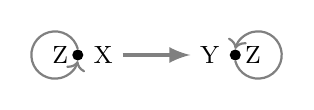
\begin{tikzpicture}
                \node[circle, fill, minimum size =4, inner sep = 0, label={[name=left]right:{\small X}}](L) at (-1,0) {};
                \node[circle, fill, minimum size =4, inner sep = 0, label={[name=right]left:\small Y}](R) at (1,0) {};
\draw[ultra thick, -latex, gray] (left.east) --  (right.west);
\draw [thick, ->, gray] (L.north)arc(15:345:0.3);
                                    \node[left, black] at (L) {\small Z};
                                    \draw [thick, ->, gray] (R.south)arc(-165:165:0.3);
                                    \node[right, black] at (R) {\small Z};

        \end{tikzpicture}}
        \fcaption{\label{derbyklassenline}}
\end{figure}\\
Straight away this can be seen to satisfy the intuitive conditions i), iii), iv) and v). Also as $X$ and $Y$ anti-commute, it is clear that every pair of edges that meet head-to-tail anti-commute, whereas pairs of edges that meet head-to-head or tail-to-tail commute. We can correct this behaviour by mapping every pair of these edges, those which currently commute but should anti-commute, to act upon a common ancillary qubit with X and Y gates respectively. Though this procedure is performed on a directed graph it still holds for edges in both directions as $E_{ij} = -E_{ji}$, so if $E_{ij}$ anti-commutes with an operator so will $E_{ji}$. Therefore, by adding ancillary qubits we can make the mapping also satisfy restriction ii).
\\\\ On a square lattice this common ancillary qubit can be the face qubit adjacent to the edges, as every pair of head-to-head or tail-to-tail edges share a common face qubit (see Fig~\ref{squareLattice}). It can be seen that using an ancillary ``face'' qubit to introduce two separate anti-commutation relations does not break the restriction iv), as long as opposite edges of black squares act in commutable ways upon the ``face'' qubit (i.e. with same gate). \\\\
\textbf{I think this section can be done better it is rather confusing and uses the same notation as the original paper}
In order to satisfy the loop condition, applying any given loop of edges needs to correspond to an identity in the fermionic Fock space. In other words this mapping is only valid for fermionic state representations that lie in the space stabilised by cycles of edges. This is shown in detail by the following reasoning (found in \cite{derbyklassen2}):
\begin{romanlist}
\item Let $M_G$ be the group of directed edges $e_{ij}$ and vertices $v_{i}$ which satisfy Eq.~\ref{edgecomm} for a given graph $G$, and $C_G$ be the directed cycles of graph $G$
\item The group of even fermionic operators $M_E$ is isomorphic to the quotient group $M_G/C_G$\  \textbf{Proof:}
        \begin{alphlist}
        \item Define the following invertible transformation for all edges and vertices in $G$:
                \begin{equation}
                        \begin{align}
                                M_G/C_G &\longleftrightarrow M_E\\
                                v_i C_G &\longleftrightarrow V_i\\
                         e_{ij}C_G &\longleftrightarrow E_{ij}
                        \end{align}
                \end{equation}
        \item $M_E$ contains all the possible edges not just those in $G$. As $G$ is connected, all edges not in $G$ can be constructed by composition of defined edge operators in $G$. Define this composition as:
                \begin{equation}
                        e_{ik} = e_{ij} \circ e_{jk} \longleftrightarrow E_{ik} = i E_{ij} E_{jk}
                \end{equation}
        \item As $M_G$ satisfies Eq.~\ref{edgecomm} for all $e_{ij}$ and $v_i$ in $G$, this holds for $M_G/C_G$, and therefore for all $E_{ij}$ and $V_{i}$ in $G$.
        \item All $E_{ij}$ not in $G$ can be decomposed into $E_{ij}$ in $G$ and the introduced phase difference will have no impact on Eq.~\ref{edgecomm}. Therefore, all edges and vertices satisfy the anti-commutation and commutation relations
        \item All cyclic paths in $G$ satisfy Eq.~\ref{loopcond} as:
                \begin{equation}
                       I = f(IC_G) = f\left( i^{n} \prod_{i=1}^n e_{p_i, p_{i+1}} C_G \right) =  i^{n} \prod_{i=1}^n E_{p_i, p_{i+1}}
                \end{equation}
                \item All cyclic paths that include edges ($\tilde E_{ij}$) not in $G$ also satisfy Eq.~\ref{loopcond} as the definition of composition adds a factor of $i$ for every edge that gets added so the total phase is preserved:
                \begin{multline}
                        i^{n+2} \prod^n_{i=0}E_{p_i,p_{i+1}} \tilde E_{p_{n-1}, p_n} \tilde E_{p_n p_{n+1}} =\\ i^{n+2} \prod^n_{i=0}E_{p_i,p_{i+1}} i E_{p_{n-1}, p_k} E_{p_k, p_{n}} i E_{p_{n}, p_l} E_{p_l, p_{n+1}}= i^{n+4} \prod^{n+4}_{i=1}E_{p_i, p_{i+1}} = I
                \end{multline}
        \end{alphlist} $\square$.
\item The quotient group $M_G/C_G$ has a faithful representation in the Hilbert subspace $U$ as:
        \begin{alphlist}
        \item The group $M_G$ has a representation $\sigma$ in the Hilbert space $\mathcal{H}$ of a system of qubits
        \item If a stabiliser of a non-trival subgroup of $\sigma$ contains all the elements of $C_G$, then can define new representation $\tau$ as:
                \begin{equation}
                        \tau (m C_G) = Proj_U \circ \sigma(m) \> \forall \> m \in M_G/C_G
                \end{equation}
                with $U$ the common +1 eigenspace of $\sigma(C_G)$.
        \end{alphlist}
\item If $\sigma$ is a representation in the multi-qubit Pauli operators $\{\pm 1, \pm i\} \times^N_i \{I_i, X_i, Y_i, Z_i\}$ then any subgroup $S$ that is abelian and does not contain $-I$ is the stabiliser of a non-trivial vector space \cite{nielsenChuang}.
\item Since $C_G$ is abelian (\textbf{Proof}), $\sigma(C_G)$ is abelian. So if $-I\>\> \cancel \in \>\>\sigma(C_G)$, $\sigma(C_G)$ is the stabiliser of the common +1 eigenspace of $\sigma(C_G)$
\item $M_G/C_G$ (and hence $M_E$) has a representation in the code space of $\sigma(C_G)$
\end{romanlist}
Therefore, the mapping we have found is valid as long as no cycle is mapped to $-I$. As all cycles on this square lattice can be decomposed into a combination of cycles around single black and white faces (\textbf{proof}), we only need to consider these stabiliser generators individually. \\\\
As shown in Fig~\ref{blackfaceloops}, looping a black face produces $-I$ meaning it cannot be in a stabilizer, however this can be fixed by simply flipping the sign of one of the four edges. Then we get $X_1Y_5Y_2 \otimes -Y_2X_5X_3 \otimes X_3Y_5Y_4 \otimes Y_4 X_5 X_1 = -X_1^2 Y_2^2 X_3^2 Y_4^2 (Y_5X_5)^2 = - (iZ_5)^2 = I$.
\begin{figure}[htbp]
\centerline{
        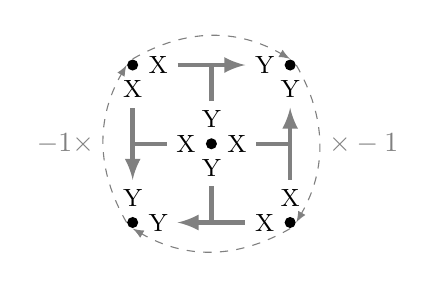
\begin{tikzpicture}
                \node[circle, fill, minimum size =4, inner sep = 0, label={[name=bottomLeftY]right:{\small Y}}, label={[name=bottomLeftY2]above:{\small Y}}](BL) at (-1,-1) {};
                \node[circle, fill, minimum size =4, inner sep = 0, label={[name=topLeftX]below:\small X}, label={[name=topLeftX2]right:\small X}](TL) at (-1,1) {};
                \node[circle, fill, minimum size =4, inner sep = 0, label={[name=bottomrightX]left:\small X},  label={[name=bottomrightX2]above:\small X}](BR) at (1,-1) {};
                \node[circle, fill, minimum size =4, inner sep = 0, label={[name=toprightY]left:\small Y}, label={[name=toprightY2]below:\small Y}](TR) at (1,1) {};
                \node[circle, fill, minimum size =4, inner sep = 0, label={[name=centreX1]left:\small X}, label={[name=centreX2]right:\small X},label={[name=centreY1]below:\small Y}, label={[name=centreY2]above:\small Y}] at (0,0) {};

                                \draw[ultra thick, latex-, gray] (bottomLeftY.east) -- node [midway](BL2BR){} (bottomrightX.west);
                                
                                \draw[ultra thick, -, gray] (centreY1.south) -- (BL2BR.center);
                                \draw[ultra thick, latex-, gray] (bottomLeftY2.north) --  node [midway](BL2TL){} (topLeftX.south);
                                \draw[ultra thick, -latex, gray] (topLeftX2.east) --  node [midway](TL2TR){} (toprightY.west);
                                \draw[ultra thick, -latex, gray] (bottomrightX2.north) --  node [midway](BR2TR){} (toprightY2.south);
                                 \draw[ultra thick, -, gray] (centreY2.north) -- (TL2TR.center);

                                  \draw[ultra thick, -, gray] (centreX1.west) -- (BL2TL.center);

                                   \draw[ultra thick, -, gray] (centreX2.east) -- (BR2TR.center);
                                   \draw[dashed,-latex, gray ] (BL.west)  to[bend left] node[left] {$-1 \times$}  (TL.west);
                                   \draw[dashed,-latex, gray] (BR.south) to[bend left](BL.south);
                                   \draw[dashed,-latex, gray] (TL.north) to[bend left](TR.north);
                                   \draw[dashed,-latex, gray] (TR.east) to[bend left] node[right] {$\times -1$} (BR.east) ;


                   \end{tikzpicture}}
           \fcaption{\label{blackfaceloops} Diagram of looping around black face. This gives $X^2 = Y^2 = I$ at every ``vertex'' qubit, but $(-X)Y(-X)Y = (XY)^2 = (iZ)^2 = -I$ at the ``face'' qubit, so overall $-I_5I_1I_2I_3I_4 = -I$. The two negative signs introduced by having to flip the orientation of the vertical edges cancel each other out.}
   \end{figure}\\
   It can be seen in Fig~\ref{whitefaceloops}, that looping a white face produces a non-trivial stabilizer, which is not $-I$. Therefore, using the mapping described (with the sign flipped on one edge of every black face) will give a faithful representation of the even fermionic algebra. \\
\begin{figure}[htbp]
\centerline{
        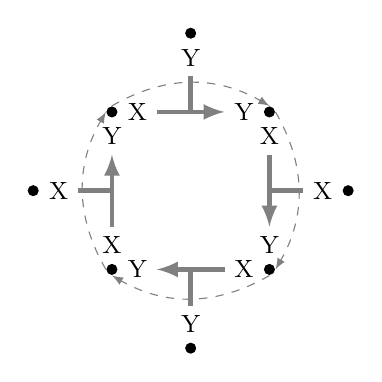
\begin{tikzpicture}
                \node[circle, fill, minimum size =4, inner sep = 0, label={[name=bottomLeftY]right:{\small Y}}, label={[name=bottomLeftY2]above:{\small X}}](BL) at (-1,-1) {};
                \node[circle, fill, minimum size =4, inner sep = 0, label={[name=topLeftX]below:\small Y}, label={[name=topLeftX2]right:\small X}](TL) at (-1,1) {};
                \node[circle, fill, minimum size =4, inner sep = 0, label={[name=bottomrightX]left:\small X},  label={[name=bottomrightX2]above:\small Y}](BR) at (1,-1) {};
                \node[circle, fill, minimum size =4, inner sep = 0, label={[name=toprightY]left:\small Y}, label={[name=toprightY2]below:\small X}](TR) at (1,1) {};
                \node[circle, fill, minimum size =4, inner sep = 0, label={[name=centreX1]right:\small X}] at (-2,0) {};
                \node[circle, fill, minimum size =4, inner sep = 0, label={[name=centreX2]left:\small X}] at (2,0) {};
\node[circle, fill, minimum size =4, inner sep = 0, label={[name=centreY2]below:\small Y}] at (0,2) {};
\node[circle, fill, minimum size =4, inner sep = 0, label={[name=centreY1]above:\small Y}] at (0,-2) {};

                                \draw[ultra thick, latex-, gray] (bottomLeftY.east) -- node [midway](BL2BR){} (bottomrightX.west);
                                
                                \draw[ultra thick, -, gray] (centreY1.north) -- (BL2BR.center);
                                \draw[ultra thick, -latex, gray] (bottomLeftY2.north) --  node [midway](BL2TL){} (topLeftX.south);
                                \draw[ultra thick, -latex, gray] (topLeftX2.east) --  node [midway](TL2TR){} (toprightY.west);
                                \draw[ultra thick, latex-, gray] (bottomrightX2.north) --  node [midway](BR2TR){} (toprightY2.south);
                                 \draw[ultra thick, -, gray] (centreY2.south) -- (TL2TR.center);

                                  \draw[ultra thick, -, gray] (centreX1.east) -- (BL2TL.center);

                                   \draw[ultra thick, -, gray] (centreX2.west) -- (BR2TR.center);
                                   \draw[dashed,-latex, gray ] (BL.west)  to[bend left]  (TL.west);
                                   \draw[dashed,-latex, gray] (BR.south) to[bend left](BL.south);
                                   \draw[dashed,-latex, gray] (TL.north) to[bend left](TR.north);
                                   \draw[dashed,-latex, gray] (TR.east) to[bend left] (BR.east) ;


                   \end{tikzpicture}}
                   \fcaption{\label{whitefaceloops} Diagram of looping around white face. }
   \end{figure}\\
Therefore, we can map the edges in the direction of their assigned orientation as:
\begin{equation}
                E_{ij} = \begin{cases}
                        X_i Y_j X_{f(i,j)} & (i,j) \text{ oriented downwards}\\
                        -X_i Y_j X_{f(i,j)} & (i,j) \text{ oriented upwards}\\
                        X_i Y_j Y_{f(i,j)} & (i,j) \text{ horizontal}\\
                \end{cases}
        \end{equation}
        with the last term ignored if the edge lies on a boundary with no adjacent face qubit. Traversing edges in the opposite direction to their orientation just involves applying a sign change. \\\\We also map the vertex operators to:
        \begin{equation}
                V_j = Z_j
        \end{equation}
        This gives a map from pauli strings to edges and vertices which in turn form a representation of the even fermionic algebra. For instance, 
        \begin{equation}
                a_1 a_2^{\dagger} + a_1^{\dagger} a_2 \longleftrightarrow - \frac{i}{2} E_{12} (V_1 - V_2) \longleftrightarrow -\frac{i}{2}X_1 Y_2 Y_{f(1,2)}( Z_1 -Z_2)
        \end{equation}
        ....., mention that it is more efficent than the other local mappings.\\
        \textbf{NEW IDEA: use (small fenwick trees) segmented bravyi-kitaev encodings combined with fermionic enumeration to improve locality}
               \section{Fermionic Enumeration}\label{fermionic-enumeration_section}
               Mitchell Chiew and Sergii Strelchuk \cite{fermionicEncoding} realised that for some of the mappings we have discussed so far there is the potential for reducing resource costs without changing anything other than the order we encode qubits. This is achieved by improving the locality of the mapping, so local operations have lower Pauli weights. In the following treatment (adapted from \cite{fermionicEncoding}) we will consider the application to the Jordan-Wigner transformation. (\textbf{waiting for new paper on applications to mappings with additional auxillary})\\\\
               In 1-D the enumeration is trivial, however, in 2D it becomes an interesting problem. For instance, consider a fermionic square lattice every mode must be assigned a qubit from a 1-D qubit array. There are many different ways of accomplishing this; most notably the S or Z pattern illustrated in Fig~\ref{SZpattern}. As discussed in Section~\ref{derby-klassen_section}, we are often interested in Hamiltonians with local interactions (e.g. between adjacent modes in the lattice). Therefore, the particular enumeration you use will impact the number of qubits that lie between neighbouring modes in the lattice. This is important as in the Jordan-Wigner transformation the Pauli-weight of a fermionic operation scales with the difference in enumeration. Thus by minimising the difference in enumeration between adjacent modes we minimise the average Pauli-weight of local interactions. This reduces to the problem of simple optimal linear arrangement (or edgesum) \cite{edgesum} from graph theory, and is formulated as:\\\\
               \textbf{Simple Optimal Linear Arrangement}: For a graph G with vertices V and edges E. Find an enumeration scheme $f: V \rightarrow \{1,2,...,n\}$ that minimises the cost function
               \begin{equation}
                       C(f) = \sum_{\alpha, \beta} |f(\alpha) - f(\beta)| \label{SOLA}
               \end{equation}
               where the average Pauli weight is given by $\frac{C(f)}{|E|} +1$.\\\\
               This problem is NP-complete \cite{edgesum} though a number of solutions are known for a range of graphs. We will consider the case of the square lattice to illustrate the principle, but it could be equally well applied to any of the other graphs with known solutions.\\\\
               The Mitchison-Durbin pattern (illustrated in Fig~\ref{mitchisondurbin}) provides the fermion enumeration scheme that minimises the average Pauli weight of hopping terms in a square lattice. Below we present a brief summary of the proof found in \cite{fermionicEncoding} and \cite{mitchisondurbin}:
               \begin{itemlist}
               \item \textbf{Lemma 7.1}: The minimum  cost will be attained by a horizontally and vertically ordered enumeration (numbering increases from left to right and from top to bottom)
                        \begin{alphlist}
                        \item It can be shown that horizontal ordering never increases the vertical contributions, and clearly always decreases the horizontal ordering
                        \item Similarly, vertical ordering can be shown to never increase the cost
                        \item It can be proven that vertical ordering preserves horizontal ordering and vice verse
                        \item Therefore, given an optimal enumeration we can apply horizontal and vertical ordering together without increasing the cost, so the minimum cost will be attained by a horizontally and vertically ordered enumeration
                                      \end{alphlist}
       \item \textbf{Lemma 7.2}: Given a horizontally and vertically ordered enumeration scheme for the lattice, the cost function for the minimum-1-sum problem is:
               \begin{equation}
                       C(f) = \sum_{\alpha\in V_b} f(\alpha) + \sum_{\alpha\in V_r} f(\alpha) - \sum_{\alpha\in V_l} f(\alpha) - \sum_{\alpha\in V_t} f(\alpha) \label{hvSOLA}
               \end{equation}
               where $V_b$, $V_r$, $V_l$ and $V_t$ are the vertices in the bottom row, right column, left column and top row respectively.\\\\
               \textbf{Proof}: As horizontally and vertically ordered every absolute sign in Eq.~\ref{SOLA} can be evaluated:
                       \begin{equation}
                               C(f) = \sum_{(\mu, \nu) \in V} f(\mu+1, \nu) - f(\mu, \nu) + f(\mu, \nu+1) - f(\mu, \nu)
                       \end{equation}
                       \begin{equation}
                       C(f) = \sum_{(\mu, \nu) \in V} f(\mu+1, \nu) - f(\mu, \nu) + \sum_{(\mu,\nu) \in V} f(\mu, \nu+1) - f(\mu, \nu)
                               \end{equation}
                               \begin{equation}
                                       C(f) = \sum_{\nu = 1}^N f(N, \nu) - f(1, \nu) + \sum_{\mu =1}^1 f(\mu, N) - f(\mu, 1)
                               \end{equation}
                               \begin{equation}
                       C(f) = \sum_{\alpha\in V_r} f(\alpha) - \sum_{\alpha\in V_l} f(\alpha) + \sum_{\alpha\in V_b} f(\alpha) - \sum_{\alpha\in V_t} f(\alpha) 
               \end{equation}
               $\square.$
       \item The Mitchison-Durbin mapping splits the lattice into three regions $U$, $V$ and $\bar U \cup \bar V$, with $U$ initially the section containing labels up to $(N,1)$ and $V$ initially containing labels from $(1,N)$. These two regions form upper- and lower- skew block-triangular sections in a vertical and horizontally ordered enumeration. The first step taken is to maximise the sum $S(U)$ of labels on the boundary of the lattice in $U$ and minimise the same sum $S(V)$ in $V$, in order to minimise $C(f)$ given by Eq.~\ref{hvSOLA}. The rules for maximising $S(U)$ are:
               \begin{alphlist}
               \item Start with the top left vertex, and start numbering by moving along every new row or column as far as horizontal and vertical ordering allows. As if the row or column is not filled maximally, then the next column or row to be filled will start with a lower enumeration, decreasing $S(U)$.
               \item Then move to the longest remaining column or row starting with the top-leftmost available vertex of the lattice. As given two columns or rows of length $b > a$ and initial enumeration $i$, filling $b$ first gives contribution $i + (i+b)$ to $C(f)$ whereas filling $a$ first gives a contribution $i + (i+a)$.
               \end{alphlist}
               By symmetry, the reverse of this process minimises $S(V)$. The final region $\bar U \cup \bar V$ should be filled with columns to maximise the labels of the top row and minimise the labels of the bottom row. This uniquely determines the minimum cost enumeration for given $U$ and $V$.
       \item It can be shown $U$ and $V$ can be optimally modified to minimise the cost. Given the length of the largest square $x$, $U$ should be restricted to rows of length $x$ till a height of $x$ above the bottom row when the length of the row should be equal to or one less than the height above the bottom row. The inverse modification should be applied to $V$. This provides the optimum edgesum for a given largest square size $x$.
       \item It can be shown that the edgesum of this enumeration is given by:
               \begin{equation}
                       C^1(f_M) = N^3 - xN^2 + 2x^2 N - \frac{2}{3} x^3 + N^2 - x N - 2N + \frac{2}{3} x \label{mdcost}
               \end{equation}
               so the Mitchison-Durbin pattern is given by the value of $x$ which minimises Eq.~\ref{mdcost}. Therefore, the Mitchison-Durbin pattern is as described above and illustrated in Fig~\ref{mitchisondurbin} with $x$ the nearest integer to $N - \frac{1}{2} \sqrt{2N^2 - 2N + \frac{4}{3}}$. 
       \item So, on a square lattice we can find an optimum enumeration pattern which leads to a reduction in the cost of Simple Optimal Linear Arrangement, and therefore minimises the average Pauli weight of hopping terms. As a simple S-pattern $f_S$ has a cost function of $C^1(f_s) = N^3 - N$, it is possible to use a computer to calculate the limiting (as $N \rightarrow \infty$) reduction in average Pauli weight of 13.9\% \cite{fermionicEncoding}.
\end{itemlist}
Therefore, using fermionic encoding it is possible to increase the locality of the fermion to qubit mapping without introducing any additional resources, and simply relabelling the qubits in the existing Jordan-Wigner mapping.
                  \section{Relative performance}\label{comparision_section}
   Each of these encodings offers various advantages and disadvantages when applied to real applications such as VQEs or phase estimation discussed in Section~\ref{applications_section}. As explained in Section~\ref{vqe_section}, the efficency of these techniques is broadly based on three factors: number of qubits required, average Pauli-weight and the number of distinct Pauli-strings in the Hamiltonian. All of the different mappings make different trade-offs between these factors.\\\\
   There are some techniques \cite{reducequbits} which decrease the number of qubits required by increasing the number of distinct Pauli-strings, however we have not covered them here. All the techniques discussed in this essay leave the number of terms in the Hamiltonian unchanged.
   \subsection{'Local' versus 'non-local' mappings}
The main trade-off at play is between the Jordan-Wigner/Bravyi-Kitaev style mappings and the 'local' (Derby-Klassen style) mappings. 'Local' mappings sacrifice an increased qubit count for drastically more localised operations. Applying a local fermionic interaction on a Jordan-Wigner or Bravyi-Kitaev mapping will take $O(N)$ and $O(\log(N))$ gates respectively, whereas on the Derby-Klassen mapping it only takes 3. This significant reduction in gate count is coupled with an increase in qubit count with Derby-Klassen requiring 1.5 qubits per fermionic mode compared to the 1 qubit per mode that Jordan-Wigner and Bravyi-Kitaev need. However, the constant gate count only holds for local interactions and performing an operation involving two arbitrary modes would scale with the diameter of the graph of local interactions. Therefore, the Derby-Klassen design scheme is only useful for Hamiltonians with local interactions, and is most effective for interactions on a regular lattice for which a mapping is known \cite{derbyklassen2}. These include all uniform tilings of degree less than 4, and the cubic lattice. 
\subsection{Bravyi-Kitaev mapping versus Jordan-Wigner mapping}
There is also an important discussion to be had about the relative merits of the Jordan-Wigner and Bravyi-Kitaev transformations. As we have discussed Bravyi-Kitaev has theoretically logarithmically superior scaling in Pauli-weights, however the experimental simulations show a more nuanced picture. It has been shown that Bravyi-Kitaev leads to a small reduction in the number of gates needed to simulate molecular Hydrogen in a minimal basis \cite{seeley}. However, for larger chemicals where we would expect the scaling advantage to grow the results are more muddled.\\\\
Tranter et al. \cite{tranter2018} preformed classical simulations of quantum phase estimation on 86 molecular systems using the Bravyi-Kitaev and Jordan-Wigner mappings. They found that with no optimisation and magnitude Trotter-ordering the Bravyi-Kitaev mapping showed a consistent improvement of up to 25\% shorter circuits, but only for molecules with more than roughly 30 spin-orbitals. This reflects the additional overhead required to implement Bravyi-Kitaev, as gates must be applied to at most $4 \log(N)+2$ qubits for every even fermionic operation (if $U(i)$, $U(j)$, $R_i$ and $R_j$ are disjoint), rather than at most $N$ qubits for Jordan-Wigner. This gives Bravyi-Kitaevv a larger prefactor and makes Jordan-Wigner more efficient for small systems. When gate optimisation (e.g. removing duplicate gates)  was introduced the Bravyi-Kitaev mapping pulled even further ahead with roughly 30-40\% shorter circuits. It is worth noting that another significant advantage of the Bravyi-Kitaev mapping is a large reduction in the number of entangling CNOT gates in exchange for a small up-tick in single qubit gates. This could make the mapping easier to implement on near-term experimental devices, as it is harder to implement 2-qubit gates.
\\\\Additionally, they showed that a large amount of the advantage afforded by Bravyi-Kitaev over Jordan-Wigner is eliminated through the use of a better Trotter-ordering. Using an optimised lexicographic\fnm{a} ordering the mappings appear equivalent for small molecules, and for some larger molecules Jordan-Wigner resulted in marginally shorter circuits and lower CNOT counts. They attributed this to the complexity of the Bravyi-Kitaev mapping reducing the linearity of the CNOT chains and so being less optimisable. It should be emphasised that the lexicographic ordering drastically reduced circuit lengths for all mappings, so the better ordering simply had more of an impact upon the Jordan-Wigner mapping rather than increasing the circuit length of the Bravyi-Kitaev mapping. This behaviour was only shown to hold for lexicographic ordering, so it is unclear how an optimum ordering in Bravyi-Kitaev would perform against an optimum ordering in Jordan-Wigner.\\\\
Finally, it was found that when using lexicographic encoding the Trotter error was lower (in some cases half) for Bravyi-Kitaev than Jordan-Wigner on small systems (large molecules of more than 30 qubits were beyond the computing power available). It was suggested that the impact of this variation in error could be large when compounded by propagation through the entire phase estimation algorithm. Therefore, if this reduction in error also holds for larger systems then in the case of lexicographic ordering the reduction in Trotter steps necessary may outweigh the small increase in circuit length to make Bravyi-Kitaev the preferable choice. \\\\
In conclusion, when given the choice between these two mappings to perform a Quantum Phase Estimation, the Bravyi-Kitaev mapping seems the most appropriate choice. For no simulation regardless of optimisation or ordering did it significantly underperform the Jordan-Wigner transformation. The only instance when it was comparable was for optimised lexicographic ordering, however this may not always be possible due to architecture restraints. 
\fnt{a}{A lexicographic ordering is essentially an alphabetic ordering with respect to the Pauli strings that make up each Hamiltonian term. This attempts to maximise cancellation of CNOT gates by changing the least number of qubits between terms. From Fig~\ref{trotterStepCircuit} it can be seen how concatenating a circuit with only the fourth qubit changed would led to two CNOTs, an $R_X^{\dagger}$ and Hadamard gate cancelling out (as $H^2 = CNOT^2 = R_X^{\dagger}R_X = I$).} 
\subsection{Fermionic enumeration}
Using an optimal fermionic enumeration can reduce circuit length without requiring any additional resources. This provides a very significant speed up to the Jordan-Wigner mapping. For instance, using the Mitchison-Durbin pattern on a square-lattice produces circuits 13.9\% shorter than using an S-pattern \cite{fermionicEncoding}. Currently, fermionic enumeration schemes have only been shown to give an improvement in Jordan-Wigner mappings. Thus they might shift the balance and make Jordan-Wigner mappings (with optimum fermionic enumeration) preferable to Bravyi-Kitaev mappings. However, simulations will need to be carried out to verify this. It is important to note that fermionic encodings are only maximally efficient for interaction graphs that have known minimum edgesum solutions, however, there are other graphs for which a good enumeration scheme can also lead to an order-of-magnitude reduction in gate count.\\\\
There is current research being carried out on how fermionic encoding could improve 'local' mappings such as Derby-Klaseen. ...
\section{Conclusion}
\raggedbottom
We have discussed a number of different fermion to qubit mappings and their relative advantages. It has been shown that to optimise qubit cost a Bravyi-Kitaev mapping would likely be most effective, but there is the potential for new research into fermionic enumeration to show a Jordan-Wigner mapping should be preferred. In the current era of quantum computing with relatively small qubit counts, it is likely that optimising qubit cost will remain preferable to optimising gate cost for some time. However, if optimising gate cost is the preference we have shown that the Derby-Klassen mapping can produce constant gate costs for fermionic operators on a number of different lattice types. It remains an interesting open question whether fermionic enumeration can offer further improvements to 'local' mappings such as Derby-Klassen.
\pagebreak
\\
        \pagebreak
        \section{References}\\
\begin{thebibliography}{000}
        \bibitem{feynmann} Feynman, R.P.. {\it Simulating physics with computers}. International Journal of Theoretical Physics 1982;21(6-7):467–488. \url{doi:10.1007/bf02650179}.
        \bibitem{originalJordanWigner} Pascual Jordan and Eugene Wigner. {\it  {\"U}ber das Paulische {\"A}quivalenzverbot}. Zeitschrift fur Physik, 47(9-10):631{651, September 1928.
                \bibitem{fermionicEncoding} Chiew, M. and Strelchuk, S.. {\it Optimal Fermion-Qubit Mappings}. ArXiv:2110.12792 [Quant-Ph], 25 October 2021. \url{http://arxiv.org/abs/2110.12792}
                \bibitem{vqe}
                Tilly, Jules, Hongxiang Chen, Shuxiang Cao, Dario Picozzi, Kanav Setia, Ying Li, Edward Grant, et al. {\it The Variational Quantum Eigensolver: A Review of Methods and Best Practices}. ArXiv:2111.05176 [Quant-Ph], 9 November 2021. \url{http://arxiv.org/abs/2111.05176} \textbf{look for journal version}
                \bibitem{chemistryReview} McArdle, Sam, Suguru Endo, Alán Aspuru-Guzik, Simon C. Benjamin, and Xiao Yuan. {\it Quantum Computational Chemistry}. Reviews of Modern Physics 92, no. 1 (30 March 2020): 015003. \url{https://doi.org/10.1103/RevModPhys.92.015003}.
                \bibitem{nielsenChuang} Nielsen, M.A., Chuang, I.L.. {\it Quantum Computation and Quantum Information}. Cambridge: Cambridge University Press; 2009. ISBN
                \bibitem{seeley} Seeley, Jacob T., Martin J. Richard, and Peter J. Love. {\it The Bravyi-Kitaev Transformation for Quantum Computation of Electronic Structure}. The Journal of Chemical Physics 137, no. 22 (14 December 2012): 224109. \url{https://doi.org/10.1063/1.4768229}.

9780511976667. doi:10.1017/cbo9780511976667. 
\bibitem{suzuki} Suzuki, Masuo. {\it Generalized Trotter’s Formula and Systematic Approximants of Exponential Operators and Inner Derivations with Applications to Many-Body Problems}. Communications in Mathematical Physics 51, no. 2 (June 1976): 183–90. \url{https://doi.org/10.1007/BF01609348}.
\bibitem{bravyikitaev} Bravyi, Sergey, and Alexei Kitaev. {\it Fermionic Quantum Computation}. Annals of Physics 298, no. 1 (May 2002): 210–26. \url{https://doi.org/10.1006/aphy.2002.6254}.
\bibitem{tranter2018} Tranter, Andrew, Peter J. Love, Florian Mintert, and Peter V. Coveney. {\it A Comparison of the Bravyi-Kitaev and Jordan-Wigner Transformations for the Quantum Simulation of Quantum Chemistry}. Journal of Chemical Theory and Computation 14, no. 11 (13 November 2018): 5617–30. \url{https://doi.org/10.1021/acs.jctc.8b00450}.
\bibitem{operatorLocality} Havlíček, Vojtěch, Matthias Troyer, and James D. Whitfield. {\it Operator Locality in Quantum Simulation of Fermionic Models}. Physical Review A 95, no. 3 (29 March 2017): 032332. \url{https://doi.org/10.1103/PhysRevA.95.032332}.
\bibitem{superfast} Setia, Kanav, Sergey Bravyi, Antonio Mezzacapo, and James D. Whitfield. {\it Superfast Encodings for Fermionic Quantum Simulation}. Physical Review Research 1, no. 3 (18 October 2019): 033033. \url{https://doi.org/10.1103/PhysRevResearch.1.033033}.
\bibitem{derbyklassen} Derby, Charles, and Joel Klassen. {\it A Compact Fermion to Qubit Mapping}. Physical Review B 104, no. 3 (8 July 2021): 035118. \url{https://doi.org/10.1103/PhysRevB.104.035118}.
\bibitem{derbyklassen2} Derby, Charles, and Joel Klassen. {\it A Compact Fermion to Qubit Mapping Part 2: Alternative Lattice Geometries}. ArXiv:2101.10735 [Quant-Ph], 26 January 2021. http://arxiv.org/abs/2101.10735.
\bibitem{edgesum} Garey, M. R., D. S. Johnson, and L. Stockmeyer. {\it Some Simplified NP-Complete Graph Problems}. Theoretical Computer Science 1, no. 3 (1 February 1976): 237–67. \url{https://doi.org/10.1016/0304-3975(76)90059-1}.
\bibitem{mitchisondurbin} Mitchison, Graeme, and Richard Durbin. {\it Optimal Numberings of an $N \times N$ Array}. SIAM Journal on Algebraic Discrete Methods 7, no. 4 (1 October 1986): 571–82. \url{https://doi.org/10.1137/0607063}.
\bibitem{reducequbits} Moll, Nikolaj, Andreas Fuhrer, Peter Staar, and Ivano Tavernelli. {\it Optimizing Qubit Resources for Quantum Chemistry Simulations in Second Quantization on a Quantum Computer}. Journal of Physics A: Mathematical and Theoretical 49, no. 29 (22 July 2016): 295301. \url{https://doi.org/10.1088/1751-8113/49/29/295301}.
\bibitem{me}
                \bibitem{first}
P. Horodecki and R. Horodecki (2001), {\it Distillation and bound entanglement},
Quantum Inf. Comput., Vol.1, pp. 045-075.

\bibitem{cal}
R. Calderbank and P. Shor (1996), {\it Good quantum error
       correcting codes exist},
Phys. Rev. A, 54, pp. 1098-1106.

\bibitem{niel}
M.A. Nielsen and J. Kempe (2001), {\it Separable states are
more disordered globally than locally}, quant-ph/0105090.

\bibitem{mar}
A.W. Marshall and I. Olkin (1979), {\it Inequalities: theory of majorization and its applications},
Academic Press (New York).
\end{thebibliography}

\end{document}

